\newpage
\section{第 02 周}

\subsection{第 5 课 | 哈希表、映射、集合}

\subsubsection{脑图}

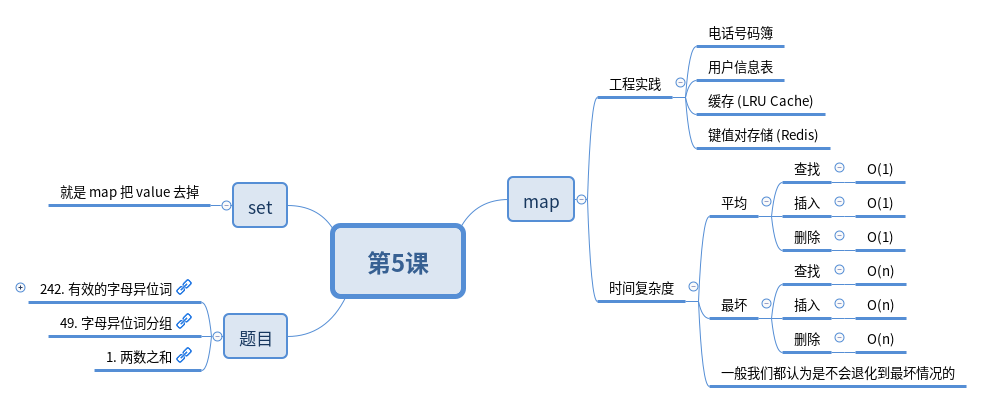
\includegraphics[width=170mm,height=80mm]{images/camp/第5课.png}

\subsubsection{题目}

\begin{itemize}
\item \hyperref[leetcode:242]{242. 有效的字母异位词}
\item \hyperref[leetcode:49]{49. 字母异位词分组}
\item \hyperref[leetcode:1]{1. 两数之和}
\end{itemize}

\subsection{第 6 课 | 树、二叉树、二叉搜索树}

\subsubsection{脑图}

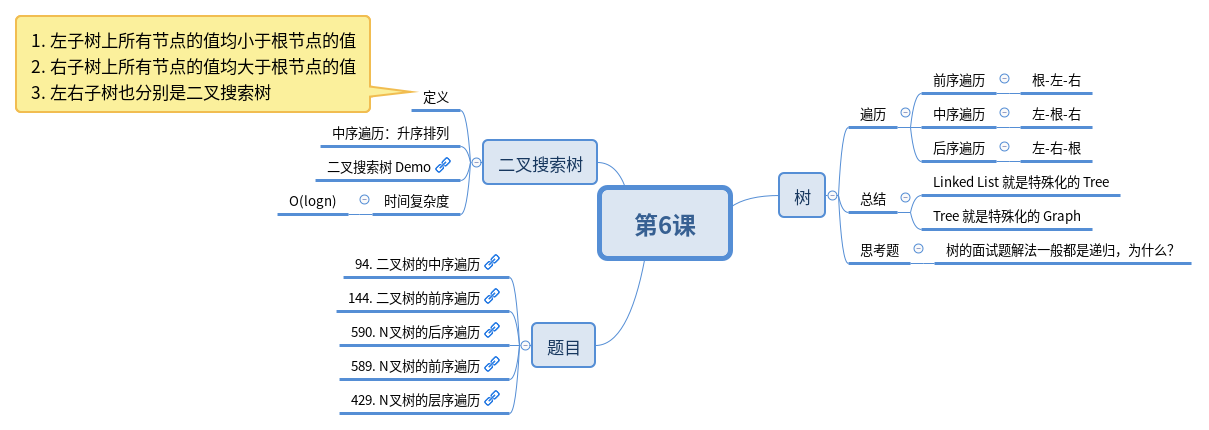
\includegraphics[width=170mm,height=80mm]{images/camp/第6课.png}

\subsubsection{题目}

\begin{itemize}
  \item \hyperref[leetcode:94]{94. 二叉树的中序遍历}
  \item \hyperref[leetcode:144]{144. 二叉树的前序遍历}
  \item \hyperref[leetcode:590]{590. N叉树的后序遍历}
  \item \hyperref[leetcode:589]{589. N叉树的前序遍历}
  \item \hyperref[leetcode:429]{429. N叉树的层序遍历}
\end{itemize}

\newpage
\section{第 7 课}

\subsection{脑图}

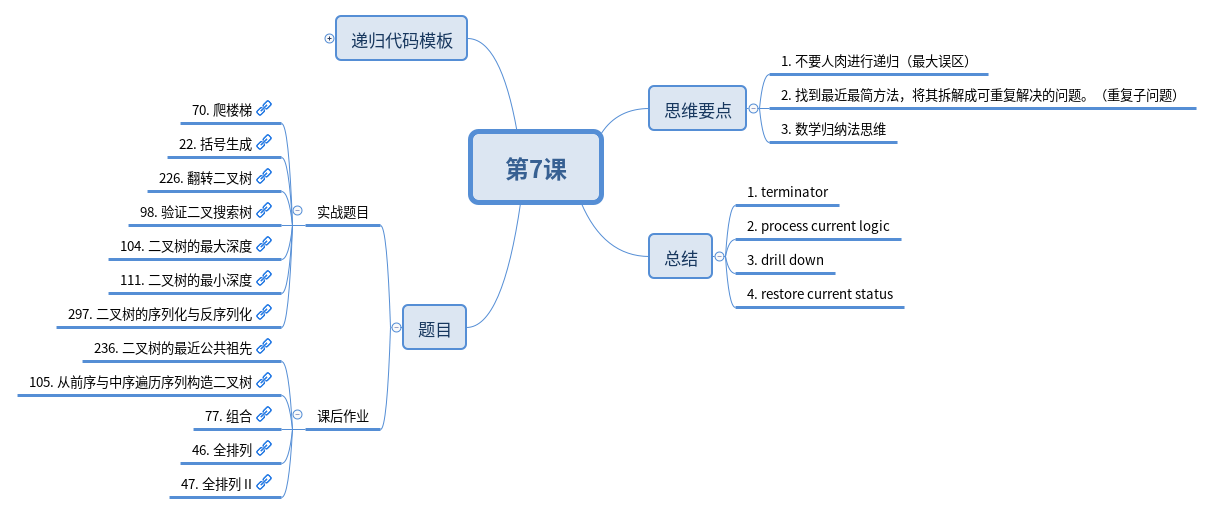
\includegraphics[width=170mm,height=80mm]{images/第7课.png}

\subsection{题目}

\subsubsection{实战题目}

\begin{itemize}
  \item \hyperref[leetcode:70]{70. 爬楼梯}
  \item \hyperref[leetcode:22]{22. 括号生成}
  \item \hyperref[leetcode:226]{226. 翻转二叉树}
  \item \hyperref[leetcode:98]{98. 验证二叉搜索树}
  \item \hyperref[leetcode:104]{104. 二叉树的最大深度}
  \item \hyperref[leetcode:111]{111. 二叉树的最小深度}
  \item \hyperref[leetcode:297]{297. 二叉树的序列化与反序列化}
\end{itemize}

\subsubsection{课后作业}

\begin{itemize}
  \item \hyperref[leetcode:236]{236. 二叉树的最近公共祖先}
  \item \hyperref[leetcode:105]{105. 从前序与中序遍历序列构造二叉树}
  \item \hyperref[leetcode:77]{77. 组合}
  \item \hyperref[leetcode:46]{46. 全排列}
  \item \hyperref[leetcode:47]{47. 全排列 II}
\end{itemize}


\subsection{学习总结}

这周学习了哈希表、集合、树、递归。

哈希表的平均时间复杂度都是 O(1) 的,所以在工程实践中被广泛使用。
大部分的语言里面都是有内置的哈希表。哈希表的最坏时间复杂度虽然
是 O(n) 的,但是一般都会设计为可自动扩容,所以一般我们都认为是
不会退化到最坏的情况的。

链表就是特殊化的树。\\
树就是特殊化的图。\\
树需要掌握前序遍历、中序遍历、后序遍历。\\
二叉搜索树的中序遍历得到的结果是有序的。\\
树这个数据结构的定义就是递归定义的,具有重复子问题,
非常适合使用递归解决树的相关问题。

递归模板:
\begin{verbatim}
// terminator
// process current logic
// drill down
// restore current status
\end{verbatim}
